%THIS IS AN EXAMPLE OF HOW YOU MIGHT INTRODUCE A CHAPTER WHICH HAS ALREADY BEEN PUBLISHED.
\cleartoevenpage
\pagestyle{empty}	%Use this to suppress the header from the preceding chapter.

\noindent
The following submitted manuscript has been incorporated as Chapter\ref{Chap:4}.

\noindent
\textbf{Wilkinson, R.D.}, Cresswell, A.G., and Lichtwark, G.A., Rock and Roll: The Influence of Bicycle Lean on the Mechanics of Non-Seated Cycling, submitted to \textit{Journal of Biomechanics} on May 26, 2020.


\begin{table}[h]
	\begin{center}
	\begin{tabular}{|c|l|l|}
		\hline
		Contributor & Statement of contribution & $\%$ \\
		\hline
		\textbf{Wilkinson, R.D.} & writing of text & 80\\
        & study design and concept & 20 \\
		& data collection & 90\\
        & data analysis & 90\\
		& statistical analysis & 100 \\
		& preparation of figures & 80 \\
		& revision of written work & 40 \\
		& supervision, guidance & 0 \\
		\hline
		Lichtwark, G.A. & writing of text & 10\\
        & study design and concept & 40 \\
		& data collection & 5 \\
        & data analysis & 5 \\
		& statistical analysis & 0 \\
		& preparation of figures & 10 \\
		& revision of written work & 30 \\
		& supervision, guidance & 50 \\
		\hline
		Cresswell, A.G. & writing of text & 10\\
        & study design and concept & 40 \\
		& data collection & 5 \\
        & data analysis & 5 \\
		& statistical analysis & 0 \\
		& preparation of figures & 10 \\
		& revision of written work & 30 \\
		& supervision, guidance & 50 \\
		\hline
	\end{tabular}
	\end{center}
\end{table}

%-------------------------------------------------------------------------------------------------------%
%-------------------------------------------------------------------------------------------------------%
%-------------------------------------------------------------------------------------------------------%
%-------------------------------------------------------------------------------------------------------%
%-------------------------------------------------------------------------------------------------------%
%-------------------------------------------------------------------------------------------------------%
%This is an internal chapter of the thesis.
%If you have a long title, you can supply an abbreviated version to print in the Table of Contents using the optional argument to the \chapter command.
\chapter[The Effect of Bicycle Lean on the Mechanics of Non-Seated Cycling]{The Effect of Bicycle Lean on the Mechanics of Non-Seated Cycling}
\label{Chap:5}	%CREATE YOUR OWN LABEL.
\pagestyle{headings}

\section{Abstract}
When riding off the saddle during climbing and sprinting, cyclists appear to coordinate the rhythmic, vertical oscillations of their centre of mass (CoM) with the side-to-side lean of the bicycle. Is the coordination of these two motions merely a stability requirement, or could it also be a strategy to more effectively generate crank power? Here we combined a kinematic and kinetic approach to understand how different constraints on bicycle lean influence CoM movement and limb mechanics during non-seated cycling. Ten participants cycled in a non-seated posture at a power output of 5 W$\cdot$kg$^{-1}$ and a cadence of 70 rpm under three bicycle lean conditions: unconstrained on rollers (Unconstrained), under instruction to self-restrict bicycle lean on rollers (Self-Restricted) and constrained in a bicycle trainer (Trainer). Bicycle lean angle in the Unconstrained condition was greater than Self-Restricted and in the Trainer. Vertical CoM displacement, peak vertical crank force, and peak instantaneous crank power in the Unconstrained condition were greater than Self-Restricted but similar to in the Trainer. The amount and rate of energy lost and gained by the rider's CoM in the Unconstrained condition was greater than Self-restricted but similar to in the Trainer. The differences in joint power contributions to total joint power (hip, knee, ankle, and upper body) between conditions were inconclusive. We interpret these results as evidence bicycle lean plays an important role in facilitating the production of high crank force and power output during non-seated cycling by allowing a greater non-muscular contribution to crank power.

\section{Introduction}
During non-seated cycling, riders lean the bicycle from side to side \autocite{Soden1978,Hull1990} in conjunction with raising and lowering their centre of mass (CoM) \autocite{Soden1978,Hull1990,Wilkinson2020b}. The bicycle leans from side to side at the same frequency as pedalling, while the CoM rises at twice this frequency. During non-seated treadmill cycling, peak lean angles of 11\textdegree from vertical have been observed and occur when each crank is close to bottom dead centre (180\textdegree) \autocite{Duc2008,Hull1990}. Studies of outdoor and ergometer cycling show the rider's CoM rises by up to 13 cm as the crank transitions from the downstroke to upstroke for each leg \autocite{Soden1978,Wilkinson2020b}. The amplitude of bicycle lean and vertical CoM displacement appear to be positively related to crank torque requirements \autocite{Soden1978,Hull1990,Duc2008,Wilkinson2020b}, but the relationship between these two motions remains unclear.

Bicycle lean is important for maintaining dynamic balance \autocite{Meijaard2007}. In the frontal plane, greater pedal forces result in greater imbalances in the moments about the line of contact between the wheels and the ground \autocite{Soden1978}. A rider can correct these imbalances using a combination of: 1) counter-steering into the fall to bring the line of contact underneath the CoM, 2) leaning the bicycle to bring the driving pedal over the line of contact, 3) generating a balancing torque at the handlebar, and 4) moving the CoM laterally \autocite{Cain2016}. Thus, maintaining dynamic balance when climbing and sprinting in a non-seated posture requires coordinated motion and a complex interaction of forces between the rider and bicycle.

Evidence suggests vertical CoM motion and upper limb muscles can amplify crank power \autocite{Wilkinson2020b} and help riders achieve greater maximal power output \autocite{Baker2002,Dore2006}. During non-seated cycling, peak pedal forces reach magnitudes close to two times bodyweight in each downstroke \autocite{Soden1978,Dorel2018a,Wilkinson2020b}. Without the action of the arms at the handlebar, vertical pedal forces greater than bodyweight result in positive work on the CoM rather than the pedal, which can cause a 22$\%$ decrease in maximal power output \autocite{Baker2002}. The arms also act to give the CoM downward velocity, resulting in the CoM losing mechanical energy at a rate equivalent to 18$\%$ (3.9 $\pm$ 0.9 W$\cdot$kg$^{-1}$) of peak instantaneous crank power \autocite{Wilkinson2020b}. Thus, using the arms to either resist or cause accelerations of the CoM is an important strategy for generating high pedal force and power output during non-seated cycling.

The use of cycling ergometers in research has limited our current understanding of optimal strategies to perform non-seated cycling at high power output. For instance, a recent study suggested a novel forward crouching posture known to limit bicycle lean during sprinting does not impair maximal power output \autocite{Merkes2020}. However, the use of an ergometer ignores lateral dynamics of the bicycle which result from forces imparted by the rider at the pedals and handlebar. Given CoM movement and arm power contribute to crank power, and bicycle lean likely influences the rise and fall of the CoM, it is unknown how self-restricting lean (e.g. by the rider) or constraining lean (e.g. by an ergometer) impacts how power is generated during non-seated cycling at high power output.

Our aim was to investigate whether changing constraints on bicycle lean would alter a rider's vertical CoM displacement and distribution of joint power during non-seated cycling. A combined kinematic and kinetic approach was used to analyse non-seated cycling at a constant power output and cadence under three bicycle lean conditions: 1) unconstrained on rollers, 2) under instruction to self-restrict bicycle lean on rollers, and 3) constrained in a bicycle trainer. Our hypothesis was formed by drawing parallels between cycling and horse riding: to reduce the amount of positive work a horse must generate during each stride cycle, jockeys reduce their own CoM displacement by performing negative work with their lower limbs \autocite{Pfau2009}. In a similar manner, we predicted cyclists would reduce their vertical CoM displacement and net knee power in an ordered fashion from constrained in a trainer to unconstrained on rollers and finally to self-restricted on rollers.

\section{Materials and methods}
\subsection{Experimental design}
Ten participants (9M/1F, age: 28 $\pm$ 8 years, height: 1.83 $\pm$ 0.09 m, mass: 76 $\pm$ 6 kg) cycled in a non-seated posture at a power output of 5 W$\cdot$kg$^{-1}$ and a cadence of 70 rpm under three bicycle lean conditions: 1) unconstrained on rollers (Unconstrained), 2) under instruction to self-restrict bicycle lean on rollers (Self-Restricted), and 3) constrained in a bicycle trainer (Trainer). All participants gave their written informed consent prior to participating in the study according to the procedures approved by the Human Ethics Committee of The University of Queensland. Each participant used the same racing bicycle (Reacto CF 907-E, Merida, Yuanlin City, Taiwan) while on the electromagnetically-braked rollers (Real E-motion B+, Elite, Fontaniva, Italy) and mounted in the trainer (Qubo Digital Smart B+, Elite, Fontaniva, Italy). Before testing, participants performed several familiarisation bouts of cycling in a non-seated posture on the rollers until they gave verbal confirmation their technique felt comfortable and was similar to riding outdoors. For safety, participants wore a helmet and shoulder harness attached via a karabiner and a slack, static rope line to an overhead gantry. The setup did not hinder the participant's ability to move their CoM or lean the bicycle. Participants wore cleated cycling shoes (SH-R070, Shimano, Osaka, Japan) clipped into the pedals (SH-R540, Shimano, Osaka, Japan). Tyre pressure was kept constant at 689 kPa (100 psi). Subjects maintained the target power output and cadence using feedback from a visual display placed in front of them. Trials were performed in a randomised order and participants were given 3-min rest between trials. For each condition, we acquired crank angle and force signals synchronously with motion capture for 10 s once the rider achieved the target power and cadence using a 16-bit A/D conversion board (USB-2533, Measurement Computing Corporation, Norton, MA) and Qualisys Track Manager software (Qualisys AB, Gothenburg, Sweden).

\subsection{Kinematics}
Three-dimensional positions of 45 passive reflective markers were collected at 200 Hz using an eight camera, opto-electronic motion capture system (Oqus, Qualisys, AB, Sweden). Reflective markers and lightweight clusters were secured to the skin using a combination of double-sided tape and self-adhesive bandage at previously described locations suitable for measuring full-body kinematics \autocite{Wilkinson2020a,Wilkinson2020b} (marker locations are shown in Figure \ref{fig:m3f1}B). For scaling purposes, a static trial was collected with the participant standing in a standard anatomical posture before commencing the trials. The heading (yaw) angle and lean of the bicycle was determined within the motion capture global coordinate system by placing three markers in a triangular pattern on the frame of the bicycle. These markers were used to create a local coordinate system for the bicycle, which allowed us to define the position and orientation of the bicycle and cranks relative to the global coordinate system. Positive lean values were defined to be counterclockwise in relation to the wheel-ground axis when viewing the bicycle from the front. A diagram of the reference coordinates and other physical quantities is provided as Figure \ref{fig:m3f1}A.

\subsection{External forces}
Tangential and radial forces at the left and right crank, as well as crank angle, were recorded at 100 Hz using pre-calibrated, wireless, instrumented cranks (Axis, SWIFT Performance, Brisbane, Australia). Digital signals were transmitted wirelessly to a base receiver before being converted to an analogue signal through the A/D Board. Crank angle and force signals were synchronized with motion capture trajectories using the internal sampling factor within Qualisys Track Manager software. A multi-axis, dynamic calibration of each crank was performed by the manufacturer. In addition, and prior to testing, the calibrated output voltage for the tangential and radial force was verified by suspending a 2.5 kg mass from each pedal spindle with the cranks in both horizontal and vertical positions.

Motion capture marker trajectories, crank forces, and crank angles were processed using custom scripts in Matlab (R2019b, MathWorks Inc., USA). These scripts filtered crank force signals and marker trajectories with a zero-lag, second-order, low-pass Butterworth filter with a cut-off frequency of 12 Hz \autocite{Kristianslund2012}. The radial and tangential forces at each crank were transformed from the crank coordinate system to the global coordinate system based on the crank orientation \autocite{Wilkinson2020b}. Bicycle lean angle was not accounted for in these calculations. As the cranks did not measure lateral force, it is possible the true vertical crank force was greater than recorded when the bicycle was leant away from vertical, which would overestimate vertical handlebar forces. However, given peak lean angles were less than 6\textdegree, the maximum magnitude of this error is likely to be less than 1$\%$. Net vertical handlebar force was resolved as the difference between the total vertical force required to cause the measured acceleration of the rider's CoM and the sum of vertical force at the left and right cranks. Further details of this method can be found in our previous work \autocite{Wilkinson2020a,Wilkinson2020b}.

\subsection{Mechanical energy and power}
OpenSim software \autocite{Delp2007} was used to create participant-specific models by scaling segment lengths and segment masses of a previously developed generic full-body musculoskeletal model \autocite{Rajagopal2016} based on each participant's anthropometry. Inverse dynamic analysis was used to calculate hip, knee, and ankle net joint moments by combining inverse kinematic results with reaction force at the left and right cranks \autocite{Seth2011}. Individual joint power contributions were calculated as a percentage of total joint power. Inclusion of data required the cyclist to simultaneously match the target power ($\pm$ 5$\%$) and cadence ($\pm$ 5$\%$) for a minimum of five crank cycles. Cycles containing more than five samples of outlying data (>3 Median Absolute Deviations), typically due to crank signal dropout,  were detected and removed from each trial \autocite{Leys2013}, resulting in an average of eight crank cycles being analyzed for each participant in each condition.

At each instant, total joint power generated by the rider (\textit{P}$_{tot}$) is equal to the sum of crank power (\textit{P}$_{cranks}$) and the rate of mechanical energy lost or gained by the rider's CoM (\textit{P}$_{CoM}$) \autocite{VanIngenSchenau1990b}.

\begin{equation}
    P_{tot} = P_{cranks} + P_{CoM}    
    \label{eq:Ptot3}
\end{equation}

\textit{P}$_{cranks}$ was calculated as the summed product of torque and angular velocity measured at each crank. \textit{P}$_{CoM}$ was calculated using inverse kinematic results as the change in total mechanical energy (potential + kinetic) divided by the change in time. 

\begin{equation}
    P_{lb} + P_{ub} = P_{cranks} + P_{CoM}
    \label{eq:Plb3}
\end{equation}

Lower-body joint power (\textit{P}$_{lb}$) was calculated as the summed product of net joint moments and joint angular velocities at the hip, knee, and ankle of each leg. Upper-body power (\textit{P}$_{ub}$) was assumed to be the difference between \textit{P}$_{tot}$ and \textit{P}$_{lb}$. Further details regarding the application of power equations in cycling can be found elsewhere \autocite{VanIngenSchenau1990b,Martin1998,Wilkinson2020b}. 

\begin{figure}[htbp]
    \centering
    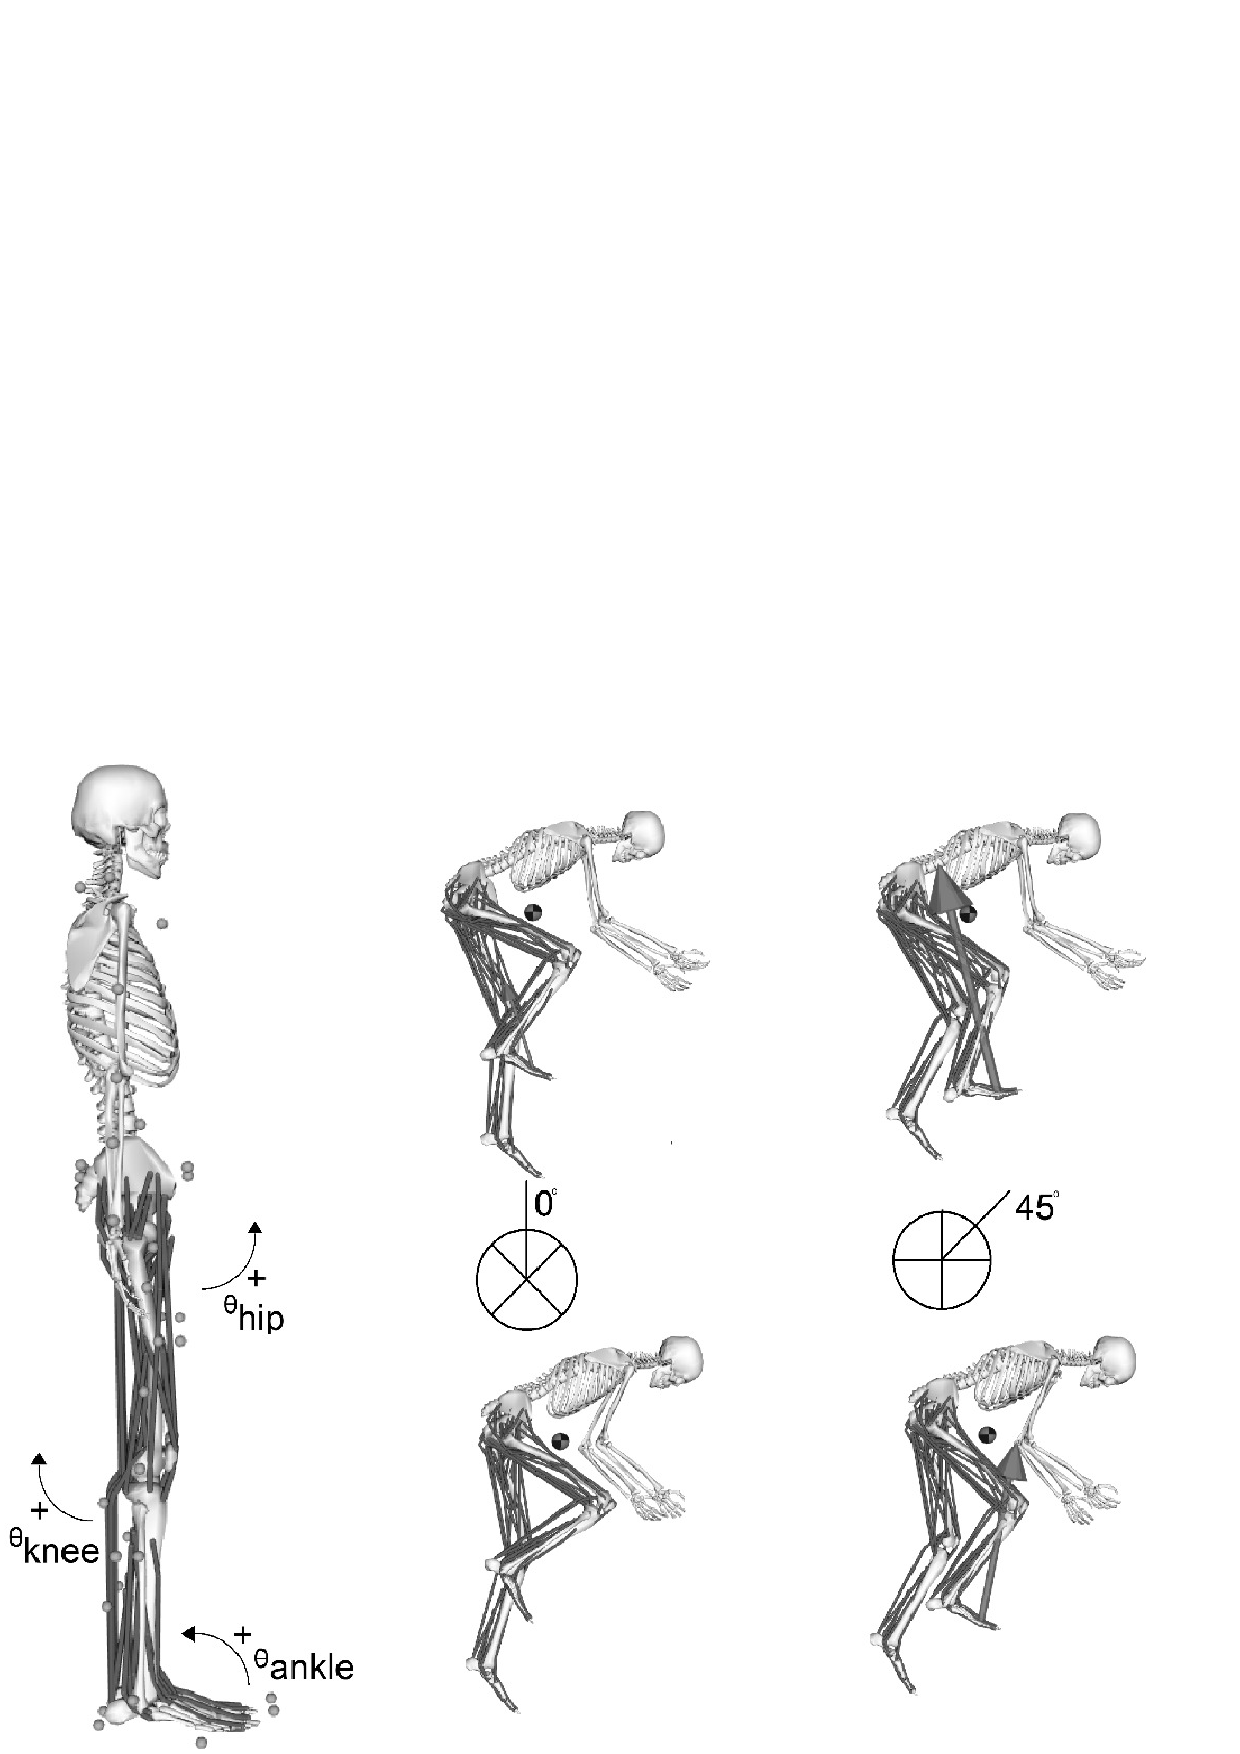
\includegraphics[width=\textwidth]{Study3/Figure1.png}
    \caption[The group mean range of bicycle lean angle in the Unconstrained condition was 54$\%$ greater than Self-Restricted and 63$\%$ greater than in the Trainer]{\textbf{The group mean range of bicycle lean angle in the Unconstrained condition was 54$\%$ greater than Self-Restricted and 63$\%$ greater than in the Trainer.} A. Front view of reference coordinates and vertical forces imparted by the rider on the bicycle. B. Diagrams depicting the musculoskeletal model cycling in a non-seated posture under the three conditions: Unconstrained, Self-Restricted, and Trainer. The group mean range of bicycle lean angle is illustrated by the arc above the rider's head. C. The group mean range of bicycle lean angle in the Unconstrained condition was 54$\%$ greater than Self-Restricted and 63$\%$ greater than in the Trainer. D. The group mean peak bicycle lean velocity in the Unconstrained condition was 20$\%$ greater than Self-Restricted and 56$\%$ greater than in the Trainer. Participant means shown in grey and the group mean in black. U, Unconstrained. S-R, Self-Restricted. T, Trainer.}
    \label{fig:m3f1}
\end{figure}
\FloatBarrier

\subsection{Statistical analyses}
We performed repeated-measures, one-way analyses of variance (ANOVAs) to test for main effects of bicycle lean condition on a number of variables (Table \ref{tab:m3t1}). The significance level was set at 0.008 prior to statistical analysis. This level was based on a desired false positive risk of $\leq$5$\%$, prior probability of 0.5, sample size of ten, and a minimum detectable effect size of 0.8 \autocite{FPRcalc}. The significance level was corrected for multiple comparisons using the Sidak method. The F-statistic (\textit{F}), p-value ($\rho$), and generalized eta squared ($\eta^2_G$) are provided for main effects. For multiple comparisons the t-statistic (\textit{t}), corrected p-value ($\rho$), 95$\%$ confidence intervals (95$\%$CI [Low to High]), and corrected effect size (\textit{Hedge's g}$_{av}$) are provided. All values are reported as mean $\pm$ standard deviation.
\FloatBarrier

%%%%%%%%%%%%%%%%%%%%%%%%%%
\section{Results}
%%%%%%%%%%%%%%%%%%%%%%%%%%
\subsection{Bicycle lean}
The range of bicycle lean (peak-to-peak) and peak lean angular velocity for each participant are presented in Figure \ref{fig:m3f1}C-D. The range of bicycle lean in the Unconstrained condition (5.6 $\pm$ 2.0\textdegree) was greater than Self-Restricted (2.6 $\pm$ 1.2\textdegree) and in the Trainer (2.1 $\pm$ 0.7\textdegree) (Table \ref{tab:m3t1}). Peak lean velocity was also greater in the Unconstrained condition (41 $\pm$ 16\textdegree s$^{-1}$) than Self-Restricted (33 $\pm$ 14\textdegree s$^{-1}$) and in the Trainer (18 $\pm$ 9\textdegree s$^{-1}$) (Table \ref{tab:m3t1}). Thus, it is likely the effects reported hereafter are predominantly due to the modification of lateral bicycle dynamics (lean) in each condition. 

\subsection{CoM motion and energetics}
Figure \ref{fig:m3f2}A-C show vertical CoM displacement, vertical CoM velocity, and vertical CoM acceleration with respect to the right crank angle in each condition. The range of vertical CoM displacement in the Unconstrained condition (5.1 $\pm$ 1.2 cm) was 24$\%$ greater than Self-Restricted (3.9 $\pm$ 1.2 cm) but similar to in the Trainer (5.3 $\pm$ 1.4 cm) (Table 1). The pattern of mechanical energy gained and lost by the rider's CoM with respect to the right crank angle is shown in Figure 3A. In each condition, phases of CoM mechanical energy loss (i.e. negative power) occurred from 55\textdegree to 155\textdegree and from 235\textdegree to 335\textdegree during the right crank cycle. Figure 4A-B show the mean range of vertical CoM displacement and the peak rate of CoM mechanical energy loss for each participant and the group in each condition. The peak rate of CoM mechanical energy loss in the Unconstrained condition (\textminus4.0 $\pm$ 1.1 W$\cdot$kg$^{-1}$) was 25$\%$ greater than Self-Restricted (\textminus3.0 $\pm$ 0.9 W$\cdot$kg$^{-1}$) but 12.5$\%$ less than in the Trainer (\textminus4.5 $\pm$ 1.3 W$\cdot$kg$^{-1}$). The peak rate of CoM mechanical energy gain in the Unconstrained condition (4.9 $\pm$ 1.2 W$\cdot$kg$^{-1}$) was 29$\%$ greater than Self-Restricted (3.5 $\pm$ 1.1 W$\cdot$kg$^{-1}$) but similar to in the Trainer (4.8 $\pm$ 1.6 W$\cdot$kg$^{-1}$).

\begin{figure}[htbp]
    \centering
    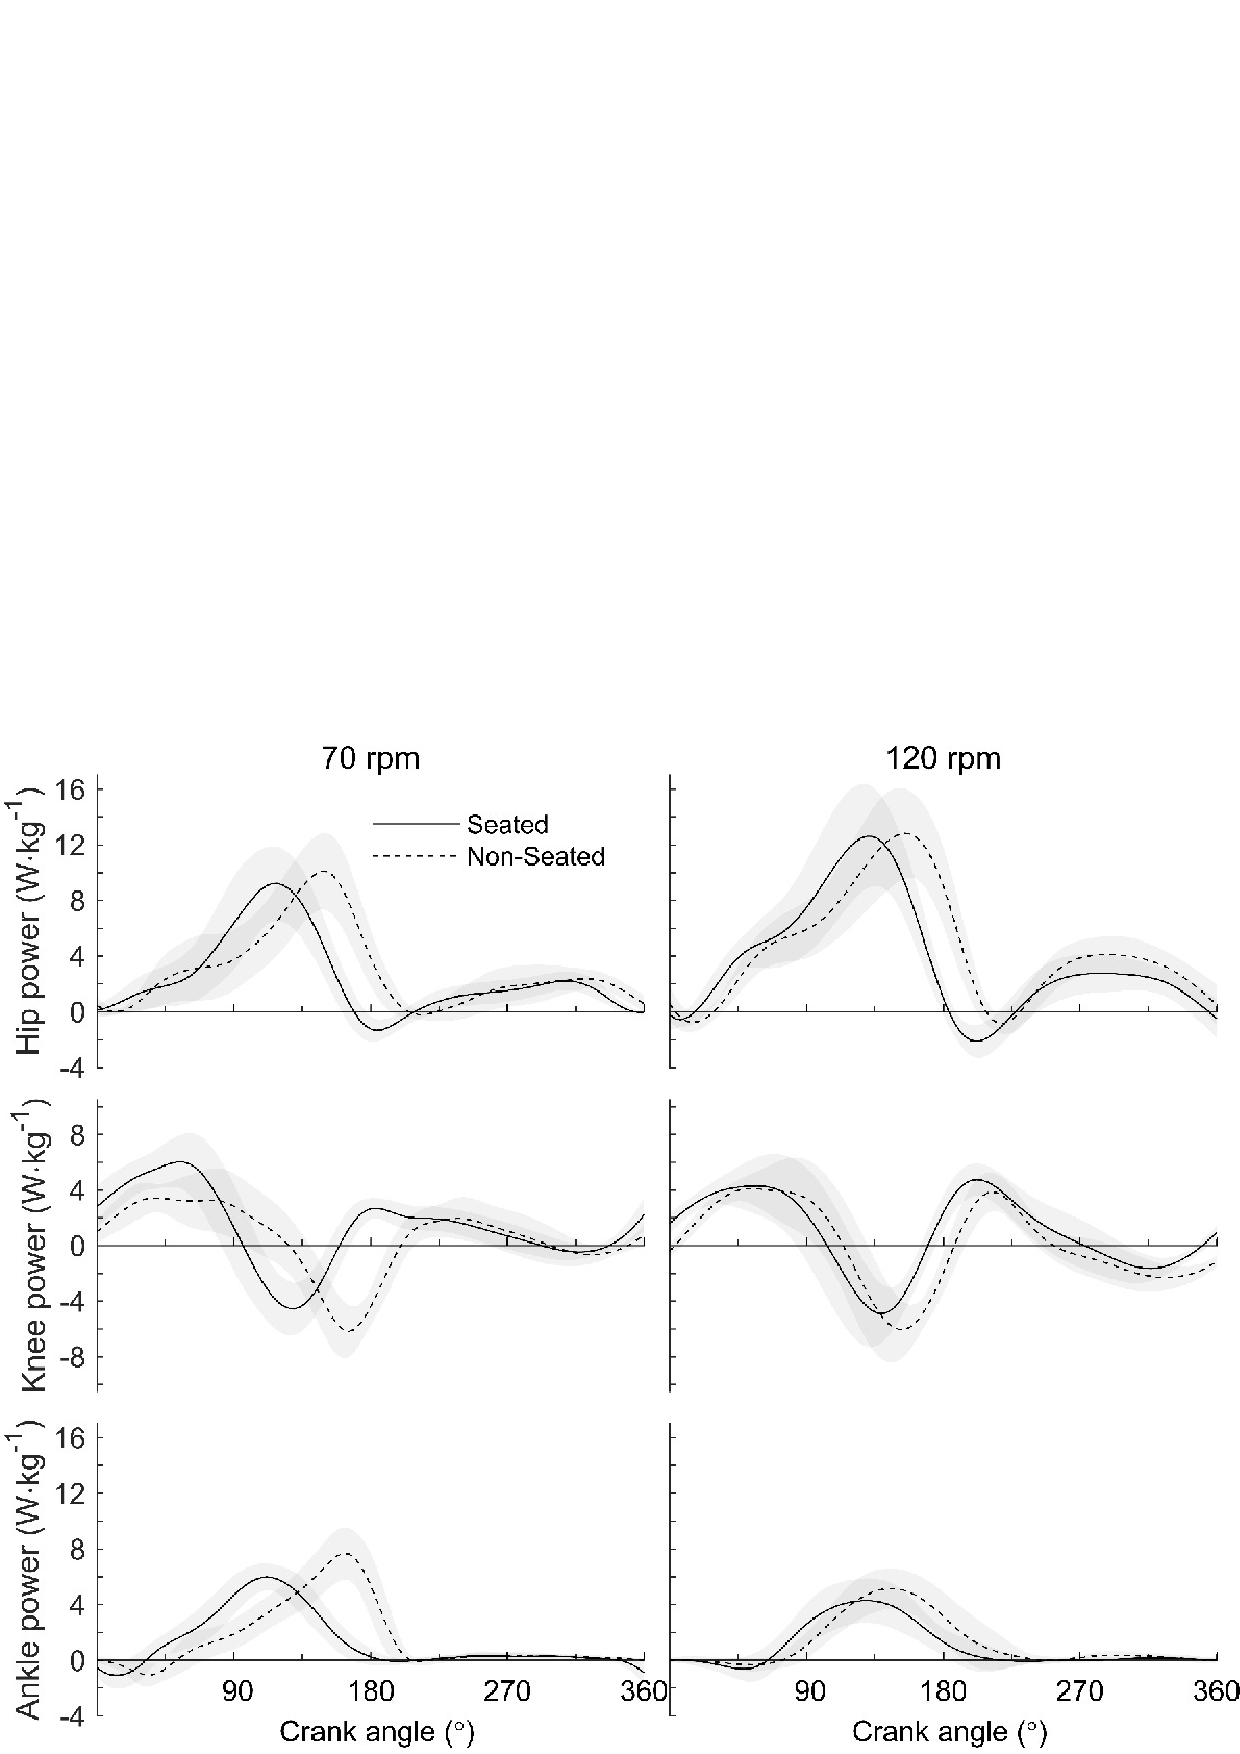
\includegraphics[width=0.6\textwidth]{Study3/Figure2.png}
    \caption[Riders self-restricted bicycle lean by reducing peak vertical forces at the crank by 15$\%$ on average.]{\textbf{Riders self-restricted bicycle lean by reducing peak vertical forces at the crank by 15$\%$ on average.} Group mean vertical CoM displacement (A), vertical CoM velocity (B), vertical CoM acceleration (C), vertical force at the left and right crank (D), and net vertical handlebar force (E) with respect to the right crank angle (0-360\textdegree) during non-seated cycling at 5 W$\cdot$kg$^{-1}$ at 70 rpm under each condition. Forces have been normalized to body weight (b.w.). In each axis (A-E), the shaded area denotes $\pm$ one standard deviation from the mean in the Unconstrained condition. Crank angles of 0\textdegree and 360\textdegree represent top dead centre position of the right crank, and 180\textdegree represents the bottom dead centre position. U, Unconstrained. S-R, Self-Restricted. T, Trainer.}
    \label{fig:m3f2}
\end{figure}
\FloatBarrier

\subsection{Vertical force}
Figure \ref{fig:m3f2}D-E show vertical crank force and net vertical handlebar force with respect to the right crank angle in each condition. Peak vertical crank force in the Unconstrained condition (122 $\pm$ 7$\%$ b.w.) was 13$\%$ greater than Self-Restricted (106 $\pm$ 6$\%$ b.w.) but similar to in the Trainer (125 $\pm$ 11$\%$ b.w.). Mean handlebar force in the Unconstrained condition (13 $\pm$ 4$\%$ b.w.) was similar to Self-Restricted (13 $\pm$ 5$\%$ b.w.) but 46$\%$ less than in the Trainer (19 $\pm$ 2$\%$ b.w.).

\subsection{Joint power}
Figure \ref{fig:m3f3}B-D show the patterns of total joint power, lower and upper body power, and individual joint power with respect to the right crank angle in each condition. Net knee power was similar between all conditions (Table \ref{tab:m3t1}). A small increase in net hip power was detected in the Self-Restricted condition (34 $\pm$ 13$\%$) compared to Unconstrained (32 $\pm$ 13$\%$). It is possible a small increase in net ankle power occurred in the Trainer condition (27 $\pm$ 7$\%$) compared to Unconstrained (24 $\pm$ 4$\%$), however our study was not sufficiently powered to detect this effect. A large variation in individual joint power contributions occurred between participants (see shaded area in Figure \ref{fig:m3f3}D). Despite the variation in individual joint power contributions between participants, there was a trend towards producing less lower body power; hence  more upper body power in the Unconstrained condition (8 $\pm$ 4 $\%$) compared to Self-Restricted (7 $\pm$ 3$\%$) and Trainer (6 $\pm$ 1$\%$), however our study was not sufficiently powered to detect this effect (Table \ref{tab:m3t1}).

\subsection{Crank power}
Figure \ref{fig:m3f3}A shows the pattern of crank power with respect to the right crank angle in each condition. Mean crank power (constrained by the task) was the same across each crank cycle (Table \ref{tab:m3t1}); hence any change in peak crank power must be compensated for at a different time during the crank cycle. For instance, peak crank power in the Unconstrained condition (11.2 $\pm$ 1.0 W$\cdot$kg$^{-1}$) was 4$\%$ higher than Self-Restricted (10.7 $\pm$ 0.8 W$\cdot$kg$^{-1}$) but similar to in the Trainer (11.6 $\pm$ 1.6 W$\cdot$kg$^{-1}$).

\begin{figure}[htbp]
    \centering
    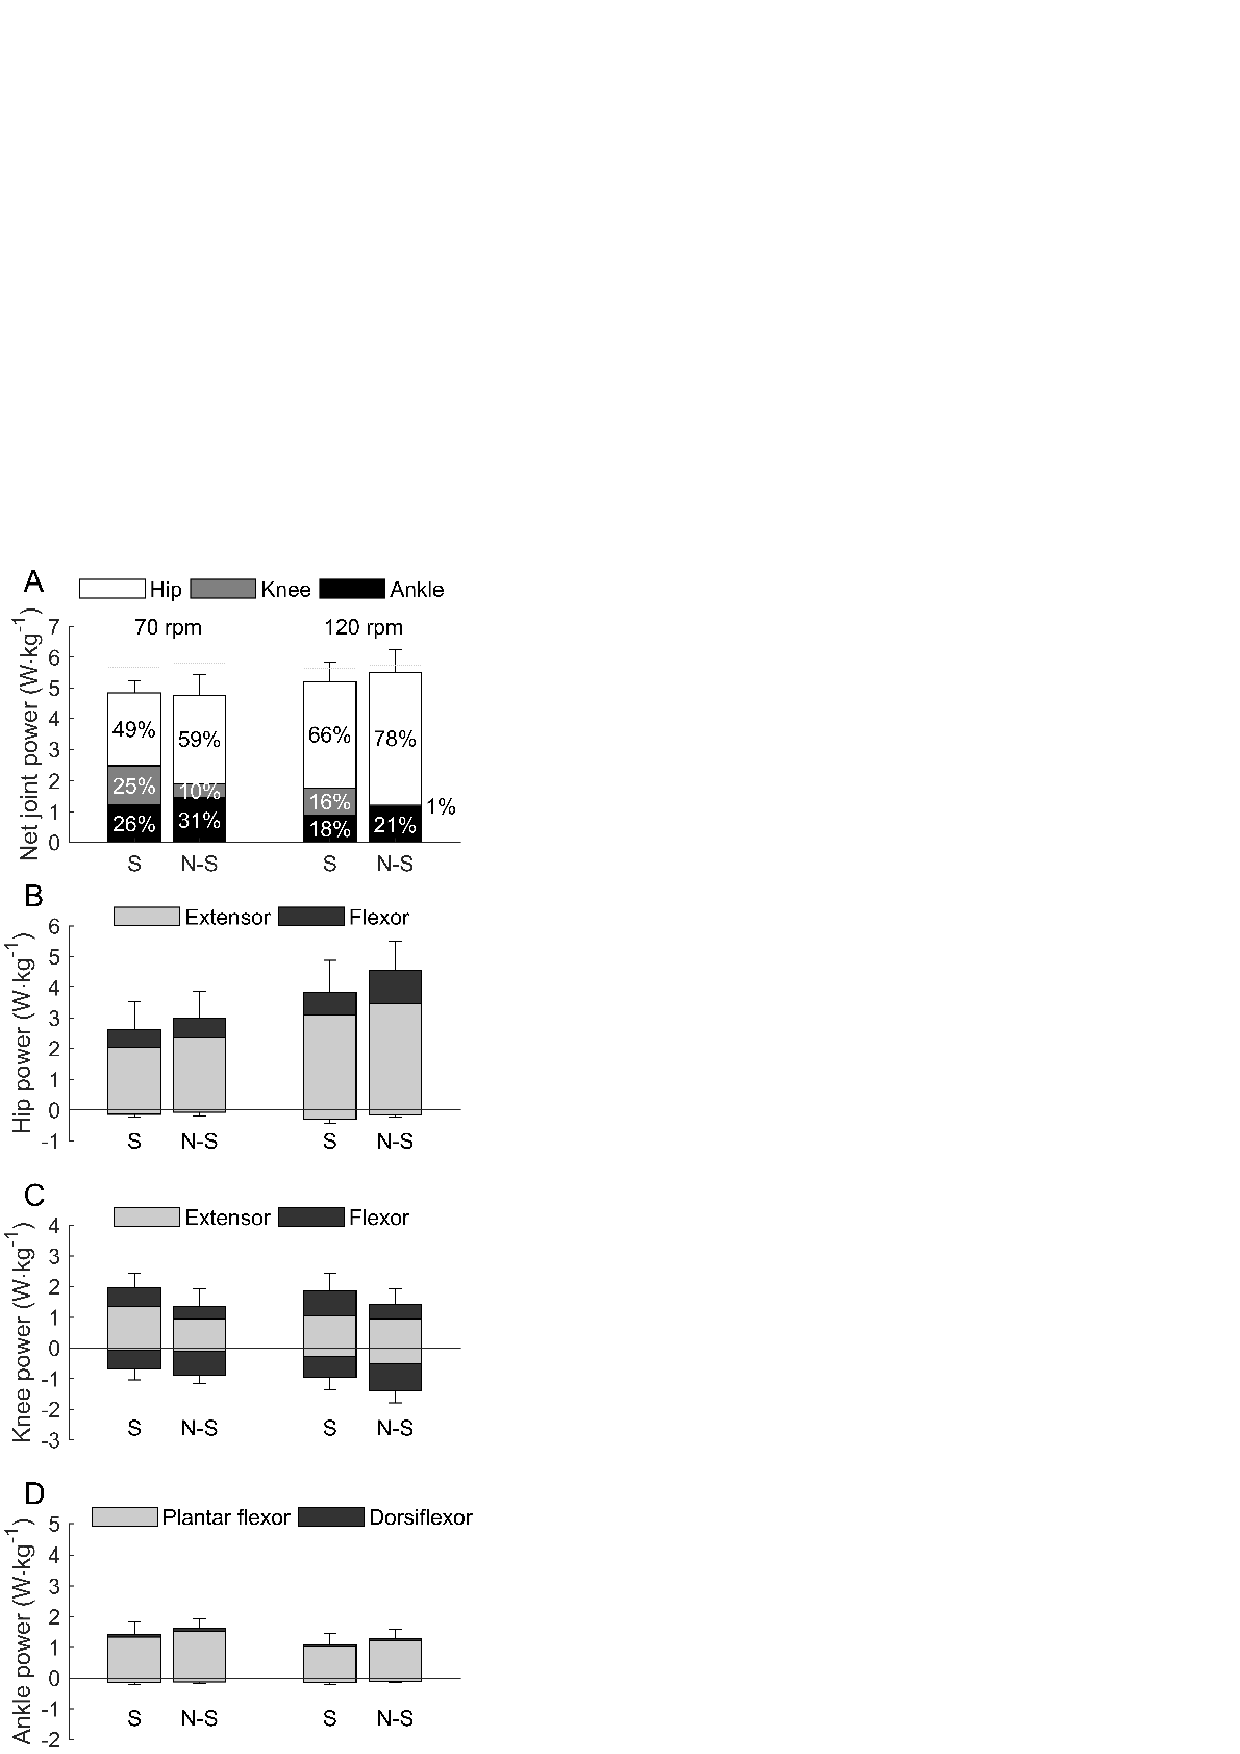
\includegraphics[width=0.65\textwidth]{Study3/Figure3.png}
    \caption[The different constraints on bicycle lean appeared to alter the pattern of total joint power production during the crank cycle]{\textbf{The different constraints on bicycle lean appeared to alter the pattern of total joint power production during the crank cycle.} A. Group mean total crank power and CoM power normalized to body mass with respect to the right crank angle (0-360\textdegree). B. Group mean total joint power normalized to body mass. C. Group mean lower body (black) and upper body power (grey) normalized to body mass. D. Group mean hip (thick black), knee (thin black), and ankle power (thin grey) of the right leg normalized to body mass. In each axis (A-D), the shaded area denotes $\pm$ one standard deviation from the mean in the Unconstrained condition. Crank angles of 0\textdegree and 360\textdegree represent top dead centre position of the right crank, and 180\textdegree represents the bottom dead centre position. U, Unconstrained. S-R, Self-Restricted. T, Trainer.}
    \label{fig:m3f3}
\end{figure}

\begin{figure}[htbp]
    \centering
    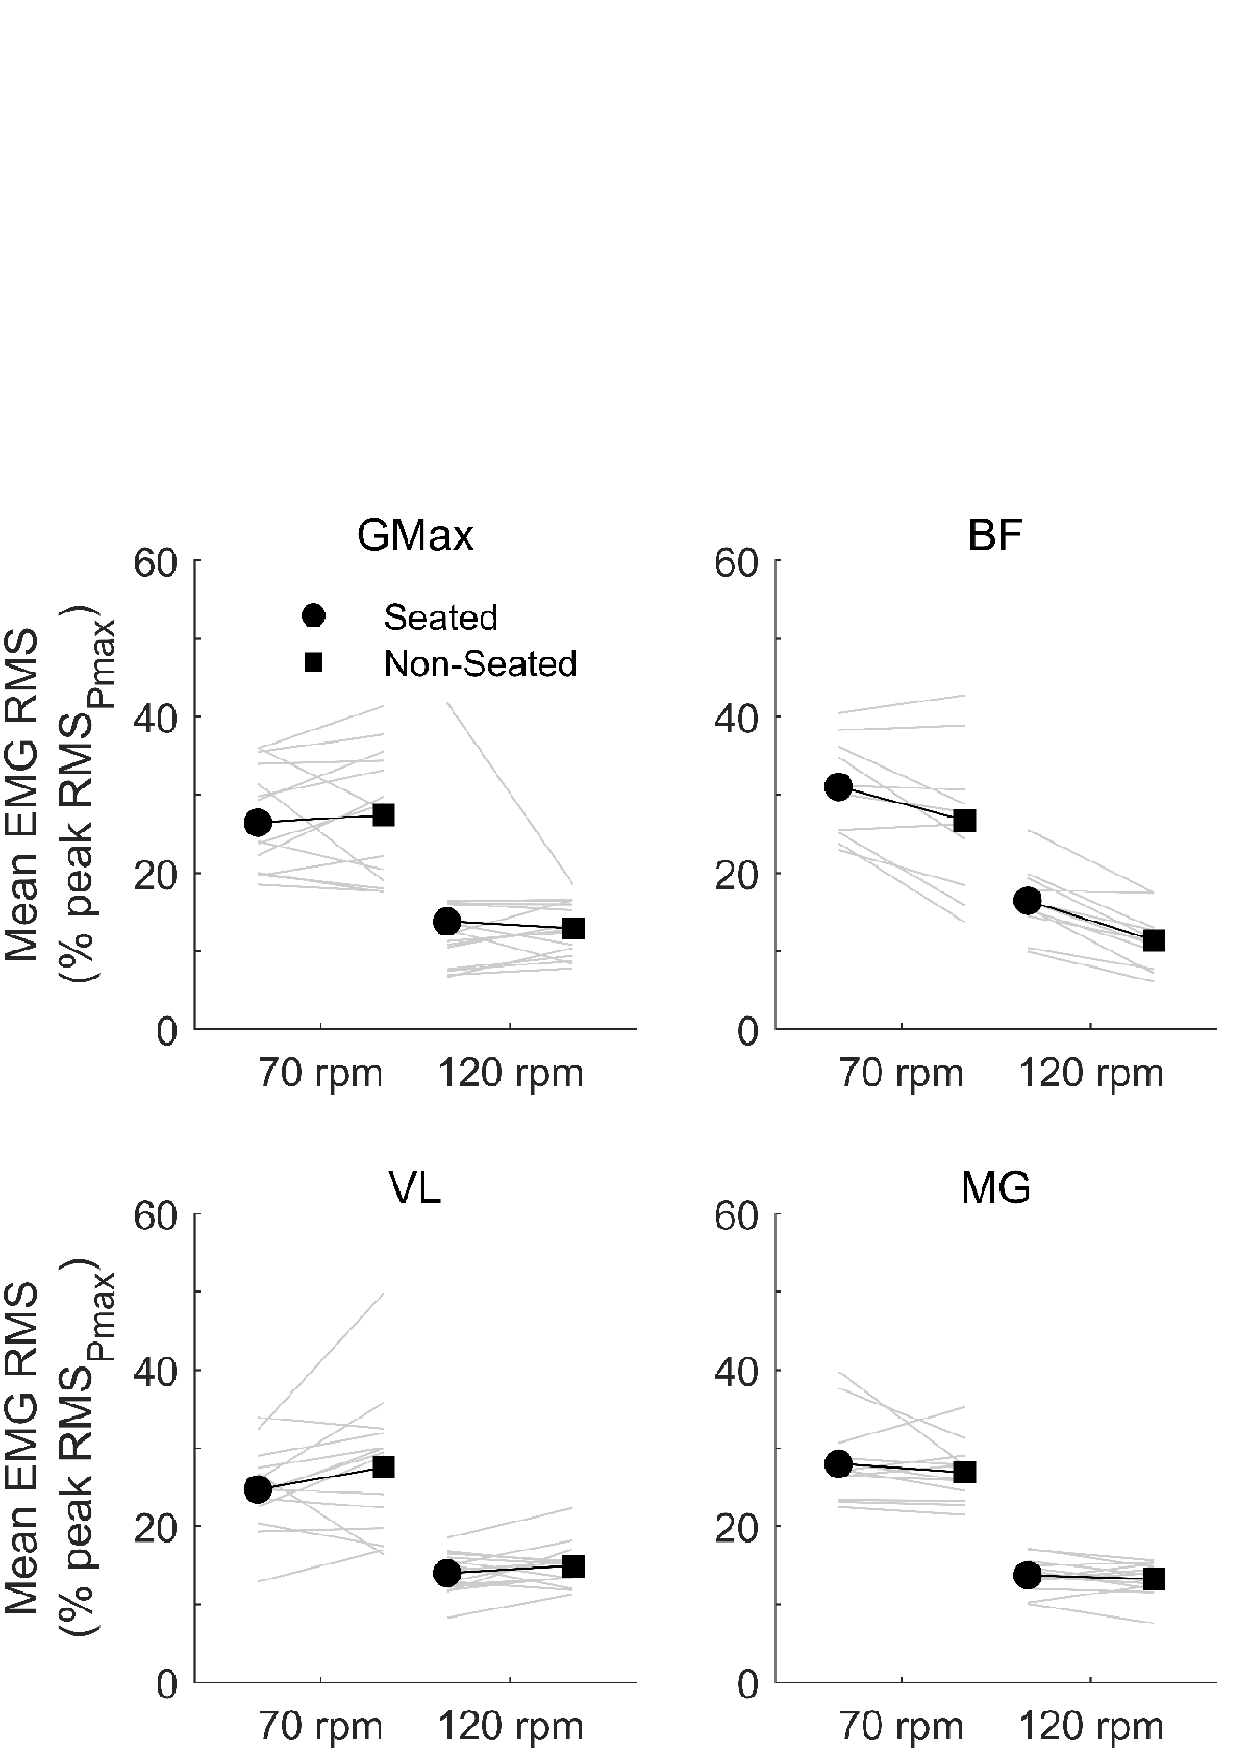
\includegraphics[width=0.65\textwidth]{Study3/Figure5.png}
    \caption[Riders increased mean and peak CoM power when lateral bicycle dynamics were constrained by a trainer, but did the opposite when having to self-restrict bicycle lean.] {\textbf{Riders increased mean and peak CoM power when lateral bicycle dynamics were constrained by a trainer, but did the opposite when having to self-restrict bicycle lean.} A. The group mean range of vertical CoM displacement in the Unconstrained condition was 24$\%$ greater than Self-Restricted, but similar to in the Trainer. B. The group mean peak rate of CoM mechanical energy loss (peak negative power) in the Unconstrained condition was 25$\%$ greater than Self-Restricted, but 12.5$\%$ less than in the Trainer. Participant means shown in grey and the group mean in black. U, Unconstrained. S-R, Self-Restricted. T, Trainer.}
    \label{fig:m3f4}
\end{figure}

\FloatBarrier

\begin{figure}[htbp]
    \centering
    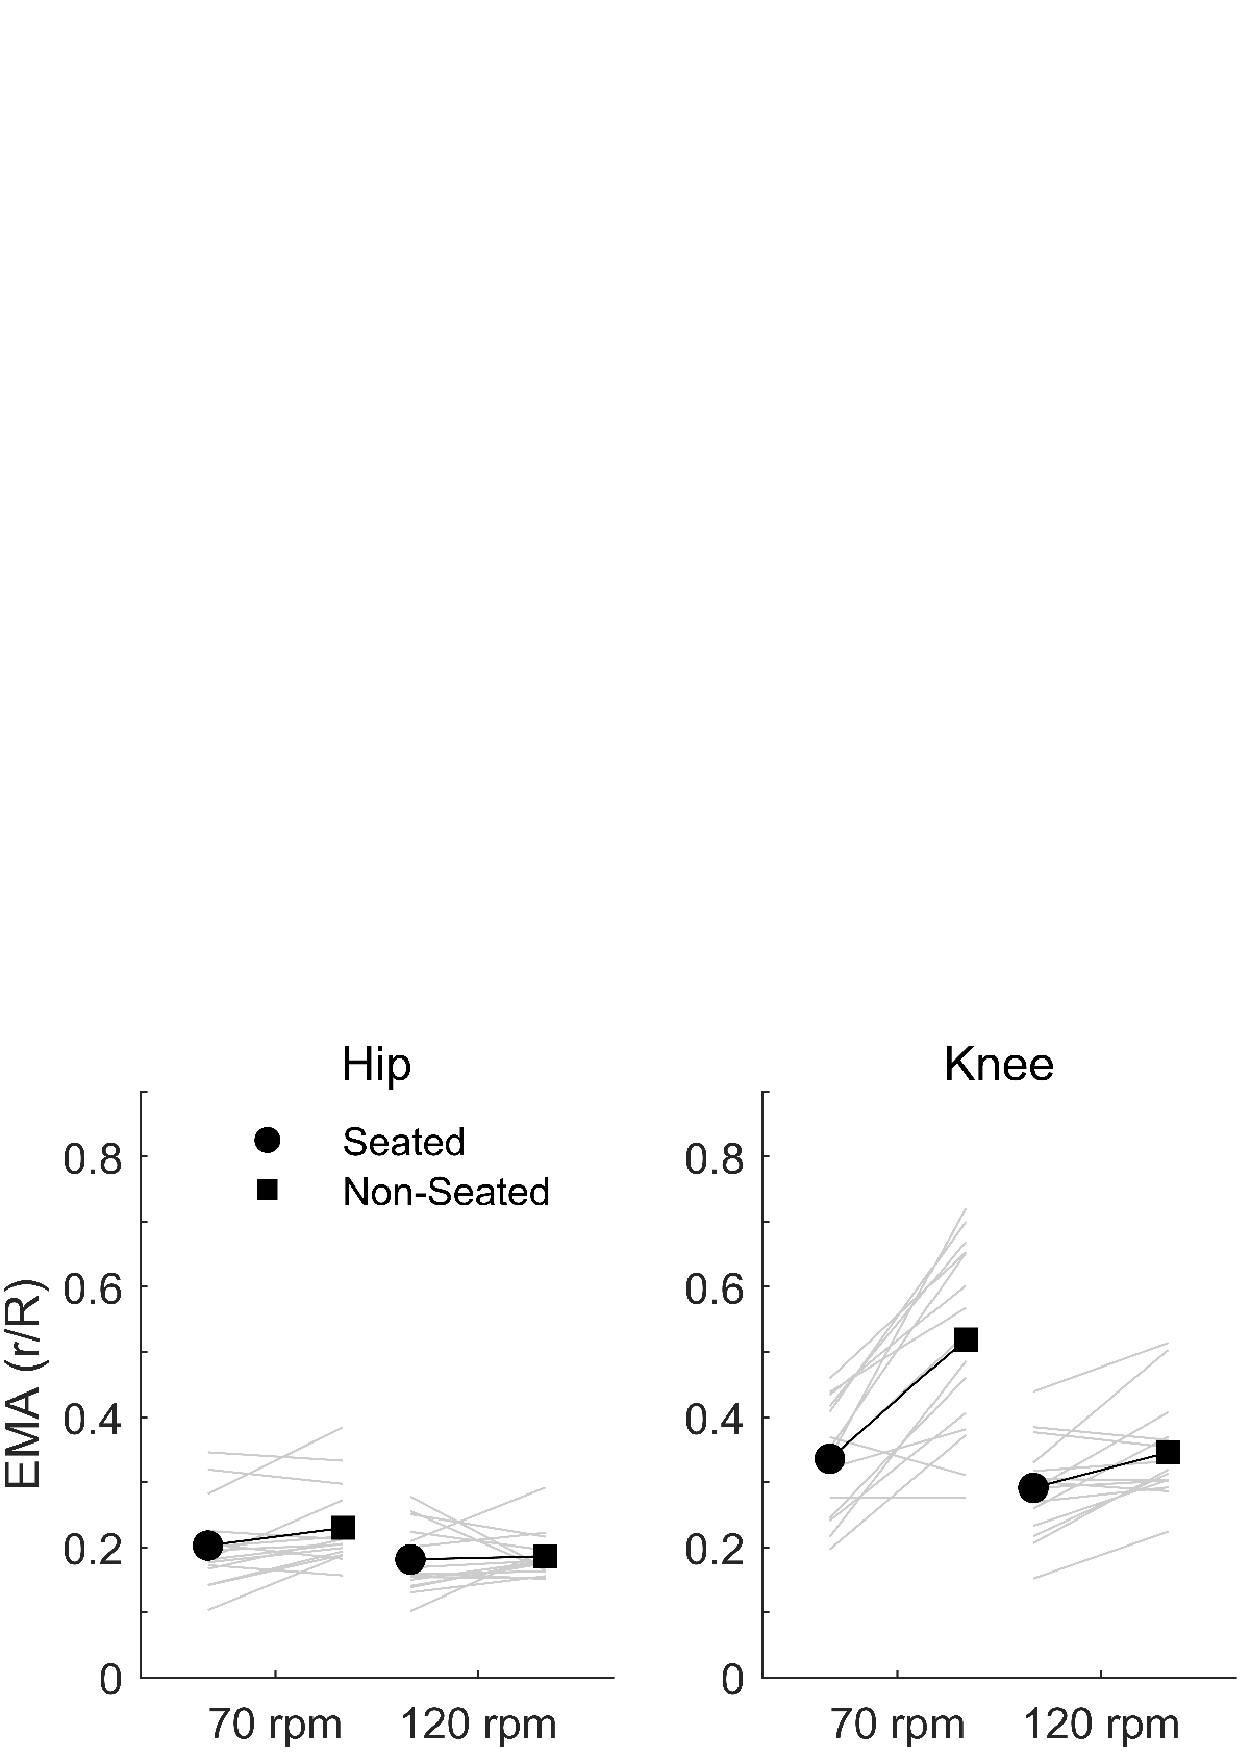
\includegraphics[width=0.65\textwidth]{Study3/Figure4.png}
    \caption[The range of bicycle lean during the unconstrained condition was less than the values reported in previous studies of non-seated cycling in the field and on a treadmill]{\textbf{The range of bicycle lean during the unconstrained condition was less than the values reported in previous studies of non-seated cycling in the field and on a treadmill.} A. Comparison of the group mean bicycle lean angle in the Unconstrained condition against data from previous literature \autocite{Soden1978,Hull1990}. B. Comparison of the group mean vertical CoM displacement in the Unconstrained condition against a rudimentary measure of lower back displacement \autocite{Soden1978} and a measure of pelvis midpoint displacement \autocite{Hull1990} from previous literature. For both comparisons, data from previous literature was extracted from published figures using Web Plot Digitizer 4.2 (\url{https://automeris.io/WebPlotDigitizer}). In each axis, the shaded area denotes $\pm$ one standard deviation from the mean in the Unconstrained condition.}
    \label{fig:m3f5}
\end{figure}

\begin{sidewaystable}
    \centering
    \includegraphics[width=\textwidth]{Study3/Table1.png}
    \caption[Self-restricting bicycle lean had a large effects on vertical crank force and CoM energetics]{\textbf{Self-restricting bicycle lean had a large effects on vertical crank force and CoM energetics.} Group results (n=10) in each condition during non-seated cycling at 5 W$\cdot$kg$^{-1}$ at 70 rpm.}
    \label{tab:m3t1}
\end{sidewaystable}

\FloatBarrier
%%%%%%%%%%%%%%%%%%%%%%%%%%
\section{Discussion}
%%%%%%%%%%%%%%%%%%%%%%%%%%
These results demonstrate that the type of constraint on bicycle lean influences a rider's vertical CoM displacement during non-seated cycling. When lean was unconstrained on rollers, the rider's vertical CoM displacement was similar to when lean was constrained by a trainer, but was significantly reduced when lean was self-restricted by the rider on rollers. Peak vertical crank force was also reduced when self-restricting bicycle lean, meaning the decrease in vertical CoM displacement also lead to a decrease in the amount and rate of total mechanical energy gain and loss by the rider's CoM. Thus, performing non-seated cycling in a bicycle trainer decouples bicycle lean from vertical CoM displacement. Given the similarity in CoM movement between the Unconstrained and Trainer conditions it seems reasonable to suggest that using greater amounts of bicycle lean had a similar effect to having a wider base of support. While the static base of support of the trainer reduces the need for stability corrections, bicycle lean appears to allow the bicycle-rider system to dynamically recover from greater perturbations around the wheel-ground axis. We interpret these results as evidence bicycle lean plays an important role in facilitating the production of high pedal force and power during non-seated cycling by increasing the magnitude of torque imbalances the bicycle-rider system can recover from.

Our results pertaining to the distribution of power between the lower and upper body were inconclusive, however there were important differences in peak and mean vertical forces between conditions. The between-participant variance in individual joint power contributions was likely a function of participants riding non-seated on rollers, which was a novel task for some and allowed multiple strategies to meet the power demands. Peak vertical crank force was highest in the Unconstrained and Trainer conditions, yet riders supported 6$\%$ more bodyweight at the cranks in the Unconstrained condition than in the Trainer. Peak vertical crank force in the Unconstrained condition was 13$\%$ greater than Self-Restricted, yet riders supported a similar amount of bodyweight at the cranks. Thus, determining how changes in bicycle lean and subsequent vertical CoM displacement influence the temporal nature of individual muscular force and work production remains a future goal.

Leaning the bicycle naturally resulted in greater vertical CoM displacement, which may have an impact on non-seated cycling performance. While increasing the work requirements to raise the CoM might be considered inefficient, our previous research suggests raising and lowering the CoM contributes significantly to peak crank power \autocite{Wilkinson2020b}. Consistent with previous research \autocite{Soden1978,Hull1990}, the results of this study show that when power output is constrained to a sub-maximal level, riders perform extra muscular work to raise the CoM as the crank transitions between the downstroke and upstroke of each leg (Figure \ref{fig:m3f2}A). This specific phasing of CoM movement means riders use mostly radial crank force and some handlebar force to perform work on the CoM, while the arms act to facilitate power transfer between the CoM and the crank during the downstroke. Future studies should investigate the impact of constraining bicycle lean and vertical CoM displacement on maximal power output and gross efficiency during non-seated cycling.

The range of bicycle lean during the unconstrained condition ($\sim$6\textdegree) was less than the values of 16-22\textdegree reported in previous studies of non-seated cycling in the field \autocite{Soden1978} and on a treadmill \autocite{Hull1990,Duc2008} (Figure \ref{fig:m3f5}A). This could be due to a number of factors. First, we conducted our study on level rollers, whereas previous studies have been on an incline. For a given power output and cadence, steeper inclines appear to result in greater amplitudes of bicycle lean \autocite{Duc2008}, which we suspect is due to the reduced inertia of the system \autocite{Fregly1996}. Second, the riding experience of our participant group was varied. Previous research shows cyclists use greater amounts of lean, rather than steering, compared to non-cyclists when on rollers \autocite{Cain2016}. Finally, there are differences between lateral bicycle dynamics on rollers compared to treadmills or in the field \autocite{Kooijman2009,Dressel2012}, thus it would be useful to conduct this study on an inclined treadmill where greater amplitudes of lean are more likely. 

In summary, we interpret our findings to suggest leaning the bicycle during non-seated cycling allows a greater non-muscular contribution to crank force and power. Further research is required to test the direct effect of bicycle lean on non-seated cycling performance.